\documentclass[aspectratio=169,14pt]{beamer}

\usepackage{fontspec}
\usepackage{graphicx}
\usepackage{xcolor}
\usepackage{array}

\setsansfont[
  Path=final_assets/fonts/,
  UprightFont=AlegreyaSans-Light.ttf,
  ItalicFont=AlegreyaSans-LightItalic.ttf
]{AlegreyaSans}
\renewcommand{\familydefault}{\sfdefault}
\usefonttheme{professionalfonts}
\setbeamertemplate{navigation symbols}{}
\setbeamertemplate{footline}{}
\setbeamertemplate{headline}{}
\setlength{\parindent}{0pt}

\definecolor{Bg}{HTML}{F0F2F5}
\definecolor{Text}{HTML}{1E2A38}
\definecolor{Dim}{HTML}{4A5568}
\definecolor{Label}{HTML}{8896A7}
\definecolor{Rule}{HTML}{CDD2D9}
\definecolor{Surface}{HTML}{E6E9EE}

\setbeamercolor{background canvas}{bg=Bg}
\setbeamercolor{normal text}{fg=Text,bg=Bg}

\newcommand{\decklabel}[1]{%
  {\fontsize{8.5}{11}\selectfont\color{Label}\MakeUppercase{#1}\par}%
}
\newcommand{\slidetitle}[1]{%
  {\fontsize{25}{30}\selectfont\color{Text}\raggedright #1\par}%
}
\newcommand{\slidebody}[1]{%
  {\fontsize{12.2}{15.4}\selectfont\color{Dim}\raggedright #1\par}%
}
\newcommand{\smallbody}[1]{%
  {\fontsize{9.5}{12}\selectfont\color{Dim}\raggedright #1\par}%
}
\newcommand{\steplabel}[1]{%
  {\fontsize{9}{11}\selectfont\color{Text}#1\par}%
}
\newcommand{\stepbody}[1]{%
  {\fontsize{9.5}{12.0}\selectfont\color{Dim}\raggedright #1\par}%
}
\newcommand{\tinynote}[1]{%
  {\fontsize{8.5}{10}\selectfont\color{Label}#1\par}%
}
\newcommand{\thinrule}{%
  \par\vspace{0.24cm}%
  {\color{Rule}\rule{2.45cm}{0.35pt}}%
  \par\vspace{0.25cm}%
}

\begin{document}

% =============================================================
% Slide 1 -- Title (Michael, 0:00-0:30)
% =============================================================
\begin{frame}[plain]
  \vspace*{0.72cm}
  \hspace*{1.22cm}
  \begin{minipage}{0.82\paperwidth}
    \raggedright
    \decklabel{CS 184 \textperiodcentered{} Spring 2026 \textperiodcentered{} Final Presentation}
    \vspace{0.62cm}

    {\fontsize{37}{44}\selectfont\color{Text}Limitless: Infinity\par}
    \vspace{0.25cm}
    {\fontsize{15.6}{20}\selectfont\color{Dim}Repulsive-surface optimization for self-intersection-free meshes.\par}
    \vspace{0.46cm}
    \textcolor{Rule}{\rule{2.45cm}{0.35pt}}
    \vspace{0.26cm}

    {\fontsize{9.5}{12}\selectfont\color{Label}
    Atharv Sampath \quad \textperiodcentered{} \quad Michael Pham
    \quad \textperiodcentered{} \quad Daniel Liu\par}
  \end{minipage}
\end{frame}

% =============================================================
% Slide 2 -- The goal / motivation (Michael, 0:30-1:00)
% =============================================================
\begin{frame}[plain]
  \vspace*{0.82cm}
  \hspace*{1.22cm}
  \begin{minipage}{0.80\paperwidth}
  \raggedright
  \decklabel{01 -- Motivation}
  \vspace{0.54cm}
  \slidetitle{Repulsive energies as self-intersection barriers.}
  \thinrule
  \slidebody{Mesh interpolation, averaging, and packing routinely produce self-intersecting outputs. The tangent-point energy makes them impossible by construction.}
  \vspace{0.30cm}
  \tinynote{Math lineage: knot energies (O'Hara, Strzelecki, von der Mosel) extended from curves to surfaces.}
  \vspace{0.10cm}
  \tinynote{Cited applications: computational anatomy, soft-body robotics, biological membranes, digital manufacturing.}
  \end{minipage}
\end{frame}

% =============================================================
% Slide 3 -- The energy (Michael, 1:00-1:25)
% =============================================================
\begin{frame}[plain]
  \vspace*{0.82cm}
  \hspace*{1.22cm}
  \begin{minipage}{0.78\paperwidth}
  \raggedright
  \decklabel{02 -- The energy}
  \vspace{0.54cm}
  \slidetitle{Discrete tangent-point energy.}
  \thinrule
  \slidebody{Pairwise kernel; diverges at self-contact.}
  \vspace{0.55cm}
  \begin{center}
  {\fontsize{14}{16}\selectfont\color{Text}
  $\displaystyle
    \widehat{\Phi}(x)
      = \sum_{t_1 \ne t_2}
        a_1 a_2 \,
        \frac{\bigl|\langle n_1,\, c_1 - c_2\rangle\bigr|^{6}}
             {\|c_1 - c_2\|^{12}}
  $%
  }
  \end{center}
  \end{minipage}
\end{frame}

% =============================================================
% Slide 4 -- Pipeline 1/4: Geometry (Daniel, 1:25-1:40)
% =============================================================
\begin{frame}[plain]
  \vspace*{0.82cm}
  \hspace*{1.22cm}
  \begin{minipage}{0.78\paperwidth}
  \raggedright
  \decklabel{03 -- Pipeline, step 1 of 4}
  \vspace{0.54cm}
  \slidetitle{Per-face centroids, normals, and areas.}
  \thinrule
  \slidebody{Centroid $c_t$, unit normal $n_t$, area $a_t$, plus per-corner Jacobians. Rebuilt once per outer iteration; reused everywhere downstream.}
  \end{minipage}
\end{frame}

% =============================================================
% Slide 5 -- Pipeline 2/4: Fast energy / BVH (Daniel, 1:40-2:00)
% =============================================================
\begin{frame}[plain]
  \vspace*{0.82cm}
  \hspace*{1.22cm}
  \begin{minipage}{0.78\paperwidth}
  \raggedright
  \decklabel{04 -- Pipeline, step 2 of 4}
  \vspace{0.54cm}
  \slidetitle{Hierarchical $\mathcal{O}(n \log n)$ acceleration via BVH and block-cluster tree.}
  \thinrule
  \slidebody{Admissible cluster pairs: $\max(\mathrm{diam}\,U, \mathrm{diam}\,V) \le \theta\,\|c_U - c_V\|$. Admissible $\to$ one rank-one cluster-aggregate term. Non-admissible $\to$ exact midpoint.}
  \vspace{0.20cm}
  \tinynote{Brute-vs-hierarchical agree to machine precision at $\theta = 0$; expected $\mathcal{O}(\theta^2)$ decay otherwise.}
  \end{minipage}
\end{frame}

% =============================================================
% Slide 6 -- Pipeline 3/4: Smooth descent (Daniel, 2:00-2:20)
% =============================================================
\begin{frame}[plain]
  \vspace*{0.82cm}
  \hspace*{1.22cm}
  \begin{minipage}{0.78\paperwidth}
  \raggedright
  \decklabel{05 -- Pipeline, step 3 of 4}
  \vspace{0.54cm}
  \slidetitle{Fractional Sobolev preconditioning at order $s = 5/3$.}
  \thinrule
  \begin{center}
  {\fontsize{14}{16}\selectfont\color{Text}
  $\displaystyle \bar{A}^{-1} \;=\; (-\Delta)^{-1}\, L^{2-s}\, (-\Delta)^{-1}$%
  }
  \end{center}
  \vspace{0.30cm}
  \slidebody{Two cotan-Laplacian solves around one fractional matvec; applied via left-preconditioned GMRES.}
  \vspace{0.18cm}
  \tinynote{GMRES iteration count stays flat under mesh refinement.}
  \end{minipage}
\end{frame}

% =============================================================
% Slide 7 -- Pipeline 4/4: Remeshing (Daniel, 2:20-2:35)
% =============================================================
\begin{frame}[plain]
  \vspace*{0.82cm}
  \hspace*{1.22cm}
  \begin{minipage}{0.78\paperwidth}
  \raggedright
  \decklabel{06 -- Pipeline, step 4 of 4}
  \vspace{0.54cm}
  \slidetitle{Dynamic remeshing for triangle quality.}
  \thinrule
  \slidebody{Per outer iteration: split edges $>\tfrac{4}{3}L_0$, collapse edges $<\tfrac{4}{5}L_0$, Delaunay flip, tangential smoothing toward the area-weighted circumcenter.}
  \vspace{0.18cm}
  \tinynote{No-foldover guard rejects collapses that would flip a face normal.}
  \end{minipage}
\end{frame}

% =============================================================
% Slide 8 -- Canonical embeddings (Atharv, 2:35-3:20) [LIVE CUT]
% =============================================================
\begin{frame}[plain]
  \vspace*{0.58cm}
  \hspace*{0.94cm}
  \begin{minipage}{0.84\paperwidth}
    \raggedright
    \decklabel{07 -- Canonical embeddings}
    \vspace{0.24cm}
    \slidetitle{Canonical embeddings, genus 0 through 5.}
    \vspace{0.28cm}
    \begin{columns}[T,totalwidth=0.84\paperwidth]
      \begin{column}{0.49\paperwidth}
        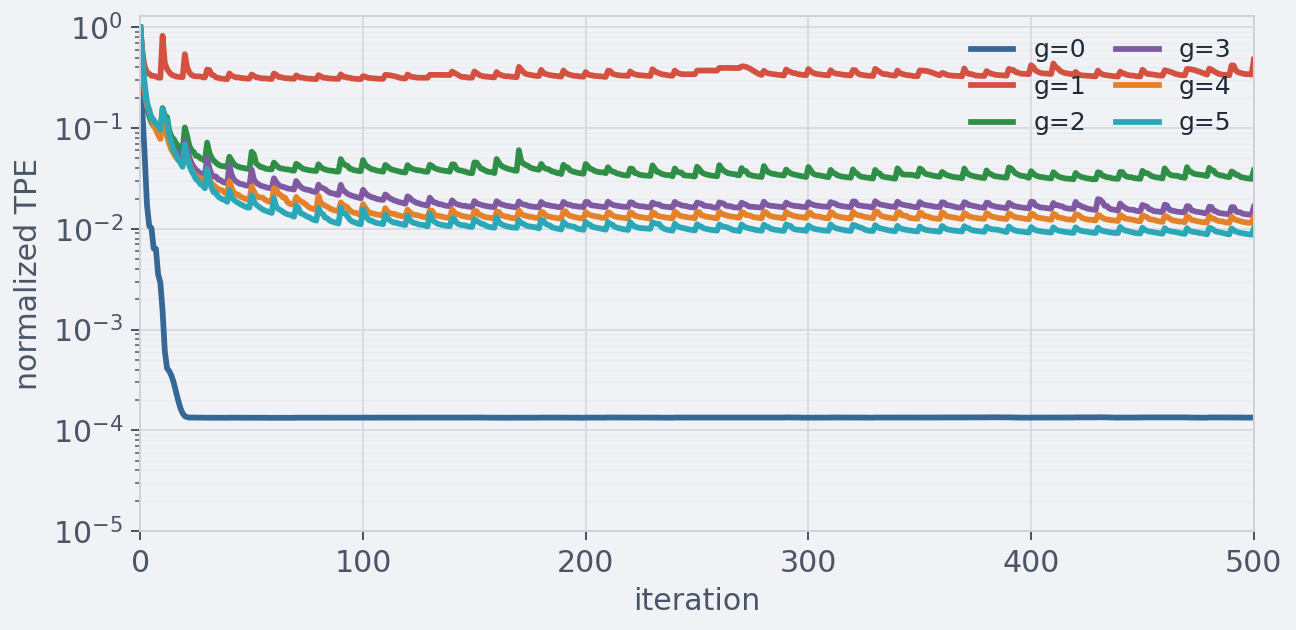
\includegraphics[width=\linewidth]{final_assets/gallery_energy_normalized.png}
      \end{column}
      \begin{column}{0.30\paperwidth}
        \smallbody{Normalized TPE, 500 iterations, genus 0 through 5.}
        \vspace{0.22cm}
        \smallbody{Genus 0 collapses to a sphere; higher genera plateau into symmetric local minima with handles intact.}
      \end{column}
    \end{columns}
  \end{minipage}
\end{frame}

% =============================================================
% Slide 9 -- Sphere through tube (Atharv, 3:20-4:05) [LIVE CUT]
% =============================================================
\begin{frame}[plain]
  \vspace*{0.58cm}
  \hspace*{0.94cm}
  \begin{minipage}{0.84\paperwidth}
    \raggedright
    \decklabel{08 -- Sphere through a tube}
    \vspace{0.24cm}
    \slidetitle{Collision-free path optimization through a tube.}
    \vspace{0.28cm}
    \begin{columns}[T,totalwidth=0.84\paperwidth]
      \begin{column}{0.49\paperwidth}
        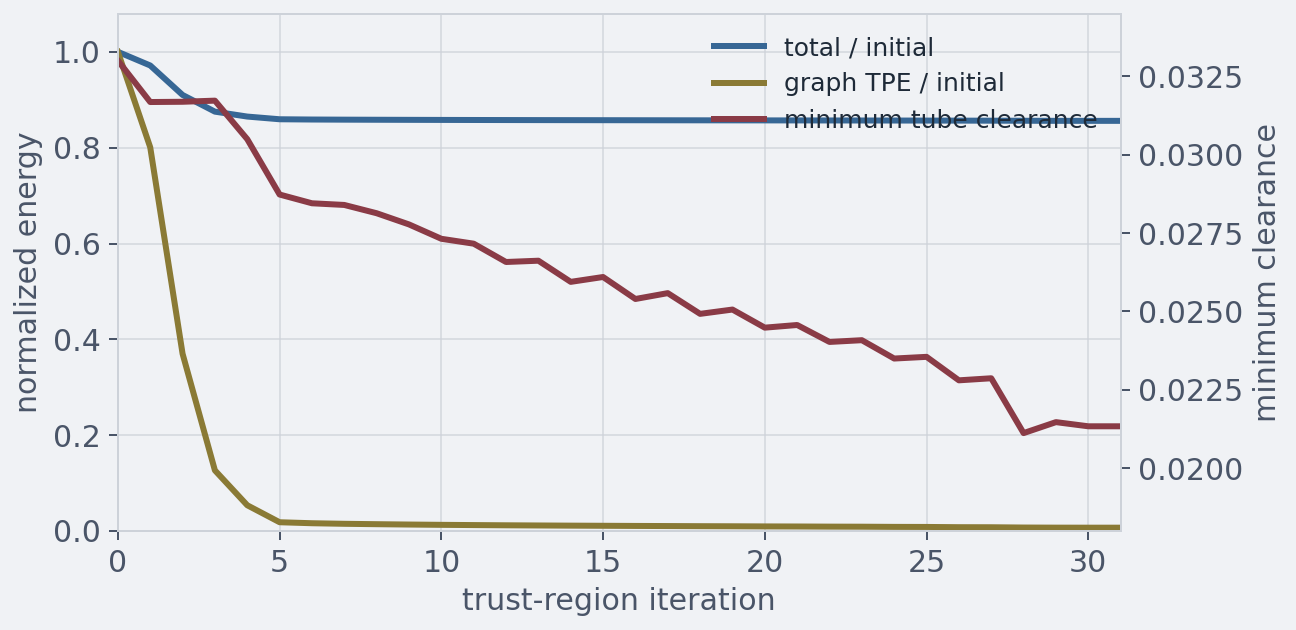
\includegraphics[width=\linewidth]{final_assets/ball_tube_energy.png}
      \end{column}
      \begin{column}{0.30\paperwidth}
        \smallbody{30-frame path, fixed endpoints. Objective: shell elasticity + self-repulsion + tube barrier.}
        \vspace{0.22cm}
        \smallbody{Self-repulsion drops two orders of magnitude in five iterations; no wall contact.}
      \end{column}
    \end{columns}
  \end{minipage}
\end{frame}

% =============================================================
% Slide 10 -- Limitations (Atharv, 4:05-4:30)
% =============================================================
\begin{frame}[plain]
  \vspace*{0.45cm}
  \hspace*{1.22cm}
  \begin{minipage}{0.82\paperwidth}
  \raggedright
  \decklabel{09 -- Limitations}
  \vspace{0.10cm}
  \slidetitle{Limitations.}
  \vspace{0.15cm}

  \renewcommand{\arraystretch}{1.4}
  \setlength{\tabcolsep}{4pt}
  \begin{tabular}{@{}p{3.4cm}p{9.2cm}@{}}
    \steplabel{CPU only} &
    \stepbody{GPU port descoped; single-threaded.} \\
    \steplabel{Cloth eversion} &
    \stepbody{Second Repulsive Shells hero demo not shipping; mid-surface init missing.} \\
  \end{tabular}
  \end{minipage}
\end{frame}

% =============================================================
% Slide 11 -- Future directions (Atharv, 4:30-4:50)
% =============================================================
\begin{frame}[plain]
  \vspace*{0.30cm}
  \hspace*{1.22cm}
  \begin{minipage}{0.82\paperwidth}
  \raggedright
  \decklabel{10 -- Future directions}
  \vspace{0.05cm}
  \slidetitle{Future directions.}
  \vspace{0.10cm}

  \renewcommand{\arraystretch}{1.0}
  \setlength{\tabcolsep}{4pt}
  \begin{tabular}{@{}p{3.4cm}p{9.2cm}@{}}
    \steplabel{Karcher means} &
    \stepbody{Multi-mesh averaging via the path solver.} \\
    \steplabel{Packing demo} &
    \stepbody{Octopus-into-box (Repulsive Shells Fig.\ 21).} \\
    \steplabel{GPU port} &
    \stepbody{Cluster-tree traversal parallelizes well.} \\
    \steplabel{Volumetric coupling} &
    \stepbody{Embed thin repulsive shells in elastic FEM solids.} \\
  \end{tabular}
  \end{minipage}
\end{frame}

% =============================================================
% Slide 12 -- Conclusion (Atharv, 4:50-5:15)
% =============================================================
\begin{frame}[plain]
  \vspace*{0.82cm}
  \hspace*{1.22cm}
  \begin{minipage}{0.78\paperwidth}
  \raggedright
  \decklabel{11 -- Summary}
  \vspace{0.54cm}
  \slidetitle{Summary.}
  \thinrule
  \slidebody{Hierarchical tangent-point energy, fractional Sobolev preconditioned descent, dynamic remeshing, graph-manifold path solver. Two end-to-end demos.}
  \vspace{0.40cm}
  \slidebody{Thanks. Happy to take questions.}
  \end{minipage}
\end{frame}

\end{document}
